\documentclass[10pt,aspectratio=169]{beamer}

\usetheme{metropolis}
\usepackage{booktabs}
\usepackage{amsmath, amssymb}
\usepackage{tikz}
\usetikzlibrary{positioning, arrows.meta, calc}
\usepackage{xcolor}
\definecolor{accent}{HTML}{3b6ea8}
\definecolor{accent2}{HTML}{c46b3a}
\definecolor{good}{HTML}{3b8a55}
\definecolor{bad}{HTML}{a04040}
\setbeamercolor{frametitle}{bg=accent, fg=white}
\setbeamerfont{frametitle}{size=\large}

\title{Predicting Reaction Success}
\subtitle{A Binary Classifier with $k$-Way Combinatorial Fusion Analysis}
\author{Gurpreet Singh \and Md Rafi}
\date{May 2026}
\institute{Machine Learning Final Project}

\graphicspath{{figures/slide/}}

% ── Helper macros ───────────────────────────────────────────────────────────
\newcommand{\fileheight}{0.75\textheight}

\begin{document}

\maketitle

% ── 1. The Problem ──────────────────────────────────────────────────────────
\begin{frame}{The Problem}
\textbf{Question: given the ingredients of a chemical reaction, will it produce
a usable amount of product?}
\vspace{0.3cm}
\begin{columns}[T,onlytextwidth]
\column{0.55\textwidth}
\begin{itemize}
\item Inputs: SMILES strings for the 6 reaction components + temperature.
\item Output: \textbf{success} (yield $\geq 50\,\%$) or \textbf{failure}.
\item Why 50\,\%: synthetic-chemistry literature's
``preparatively useful'' threshold; below it side reactions dominate.
\item Use case: \textbf{bench-chemistry triage} --- predict before running the
experiment.
\end{itemize}
\column{0.42\textwidth}
\centering
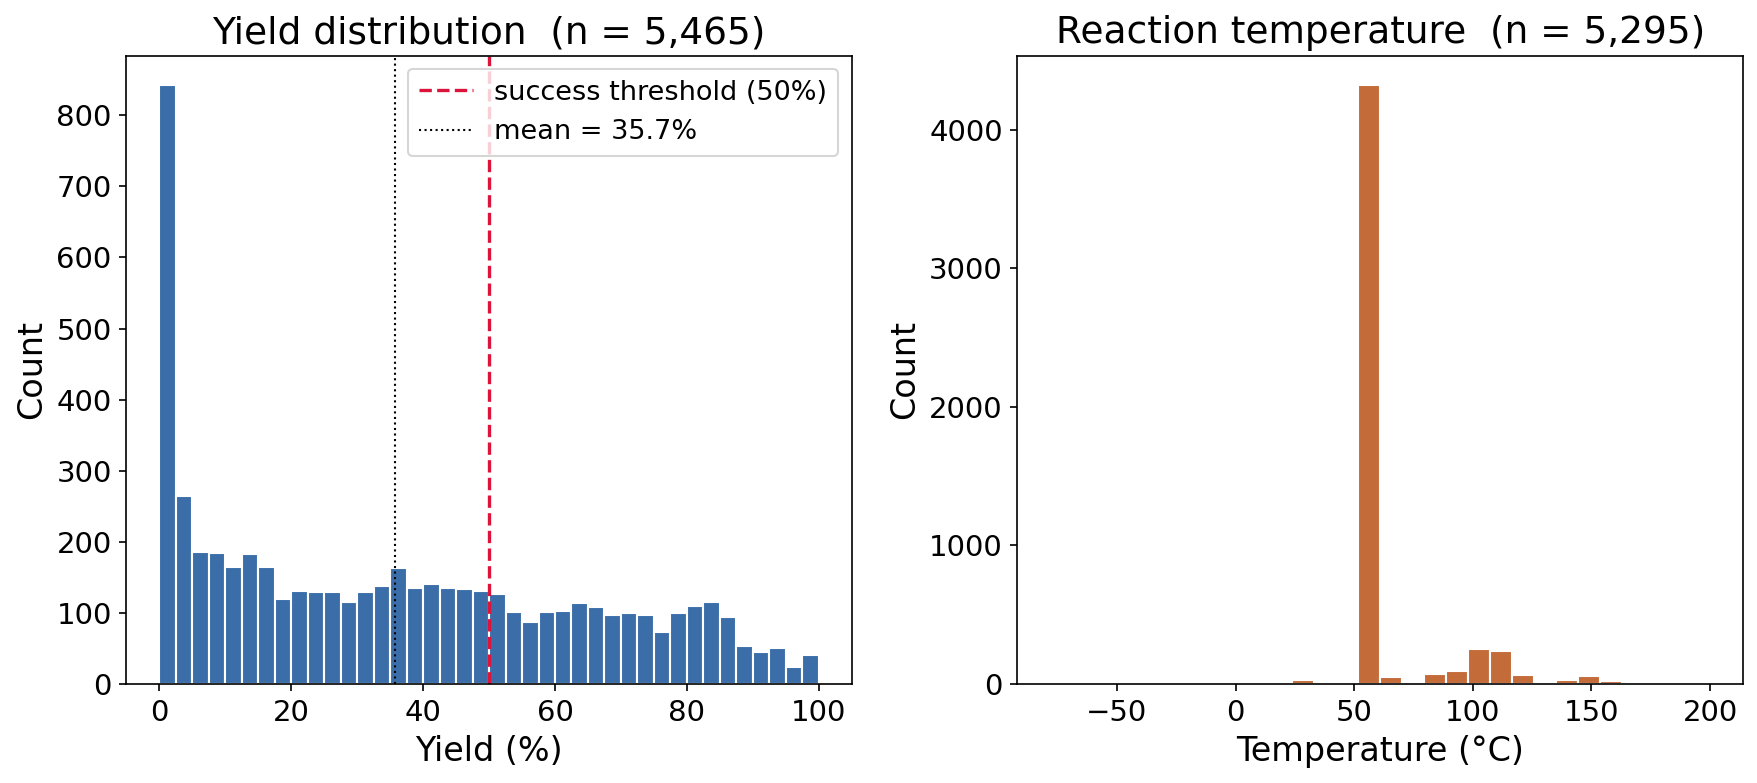
\includegraphics[width=\linewidth]{dataset_overview.png}
\end{columns}
\end{frame}

% ── 2. The pivot ────────────────────────────────────────────────────────────
\begin{frame}{Why classification, not regression?}
The first version of this project predicted continuous yield. On unseen
chemistry it \textbf{collapsed}.
\vspace{0.3cm}
\begin{itemize}
\item Random split: regression $R^2 = 0.82$ (state-of-the-art).
\item Held-out scaffolds: $R^2 < 0$ for \textbf{every} model tested.
\end{itemize}
\vspace{0.3cm}
\textbf{Why this pivot makes the project more, not less, scientifically honest:}
\vspace{0.2cm}
\begin{itemize}
\item Bench chemists make a binary decision (try / don't try); they
\emph{might not} need absolute yield precision.
\item Ranking-based ensembling (CFA) operates naturally on a binary task.
\end{itemize}
\end{frame}

% ── 3. Dataset ──────────────────────────────────────────────────────────────
\begin{frame}{Dataset}
\textbf{5,465 Buchwald--Hartwig amination reactions} from the
Open Reaction Database.
\vspace{0.3cm}
\begin{columns}[T,onlytextwidth]
\column{0.45\textwidth}
\textbf{Featurisation}
\begin{itemize}
\item 6 component-wise Morgan fingerprints
(radius 2, 2048 bits each)
\item Optional reaction-level DRFP fingerprint
\item Normalised reaction temperature
\item $\approx 14{,}337$ features per reaction
\end{itemize}
\textbf{Splits}
\begin{itemize}
\item Random 70/15/15 (in-dist)
\item Substrate-level 5-fold CV (OOD)
\end{itemize}
\column{0.5\textwidth}
\centering
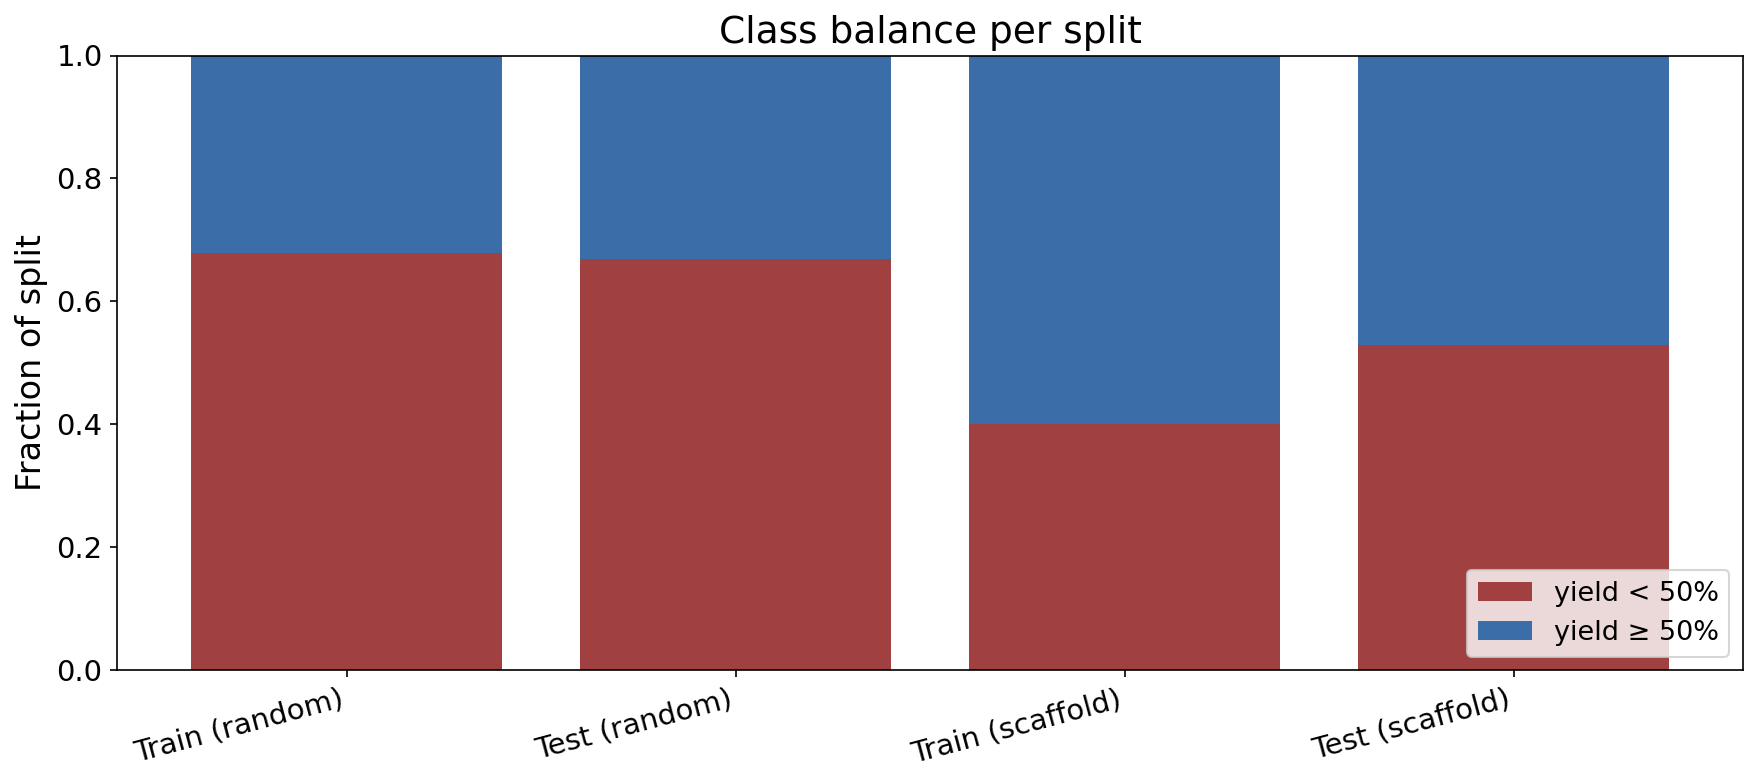
\includegraphics[width=\linewidth]{class_balance.png}
\end{columns}
\end{frame}

% ── 4. Approach ─────────────────────────────────────────────────────────────
\begin{frame}{Approach: 51-model pool + CFA}
\centering
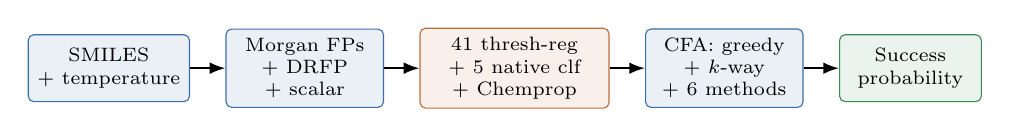
\begin{tikzpicture}[
  node distance=0.3cm and 0.45cm,
  every node/.style={font=\scriptsize},
  box/.style={rectangle, rounded corners=2pt, draw=accent, fill=accent!10,
              minimum width=2.0cm, minimum height=0.85cm, align=center},
  pool/.style={rectangle, rounded corners=2pt, draw=accent2, fill=accent2!10,
              minimum width=2.4cm, minimum height=0.85cm, align=center},
  result/.style={rectangle, rounded corners=2pt, draw=good, fill=good!10,
              minimum width=1.8cm, minimum height=0.85cm, align=center},
  arrow/.style={-{Latex[length=2mm]}, thick}
]
  \node[box] (data) {SMILES \\ + temperature};
  \node[box, right=of data] (feat) {Morgan FPs \\ + DRFP \\ + scalar};
  \node[pool, right=of feat] (pool) {41 thresh-reg \\ + 5 native clf \\ + Chemprop};
  \node[box, right=of pool] (cfa) {CFA: greedy \\ + $k$-way \\ + 6 methods};
  \node[result, right=of cfa] (res) {Success \\ probability};

  \draw[arrow] (data) -- (feat);
  \draw[arrow] (feat) -- (pool);
  \draw[arrow] (pool) -- (cfa);
  \draw[arrow] (cfa)  -- (res);
\end{tikzpicture}

\vspace{0.6cm}
\textbf{6 CFA combination methods:} ASC (mean), ARC (rank-mean),
WSCDS / WRCDS (diversity-weighted), WSCP / WRCP (performance-weighted).
\vspace{0.2cm}
\textbf{Selection}: greedy forward + exhaustive $k$-way ($k$=2..5);
val-optimal cut-off per ensemble.
\end{frame}

% ── 5. Random-split results ─────────────────────────────────────────────────
\begin{frame}{Random-split results: top models with 95\,\% CIs}
\centering
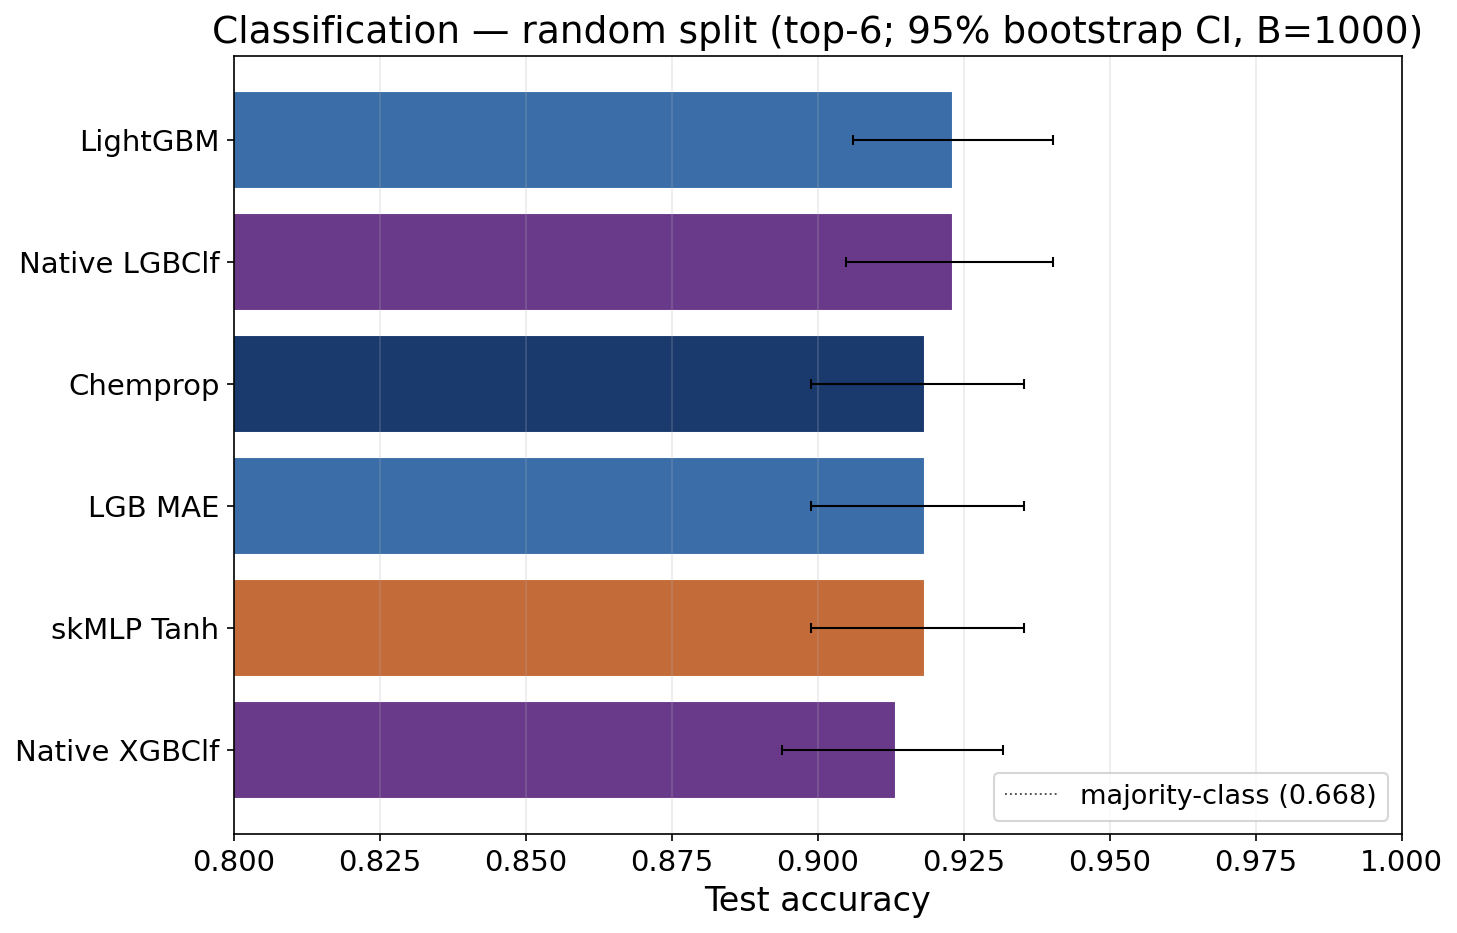
\includegraphics[width=0.95\linewidth,height=\fileheight,keepaspectratio]
{bars_classification_random.png}
\end{frame}

% ── 6. Substrate-level OOD ──────────────────────────────────────────────────
\begin{frame}{Substrate-level out-of-distribution: 5-fold CV}
\textbf{Each fold holds out a different set of unique aryl halides.}
The model never sees the test substrates during training.
\vspace{0.2cm}
\begin{columns}[T,onlytextwidth]
\column{0.55\textwidth}
\centering
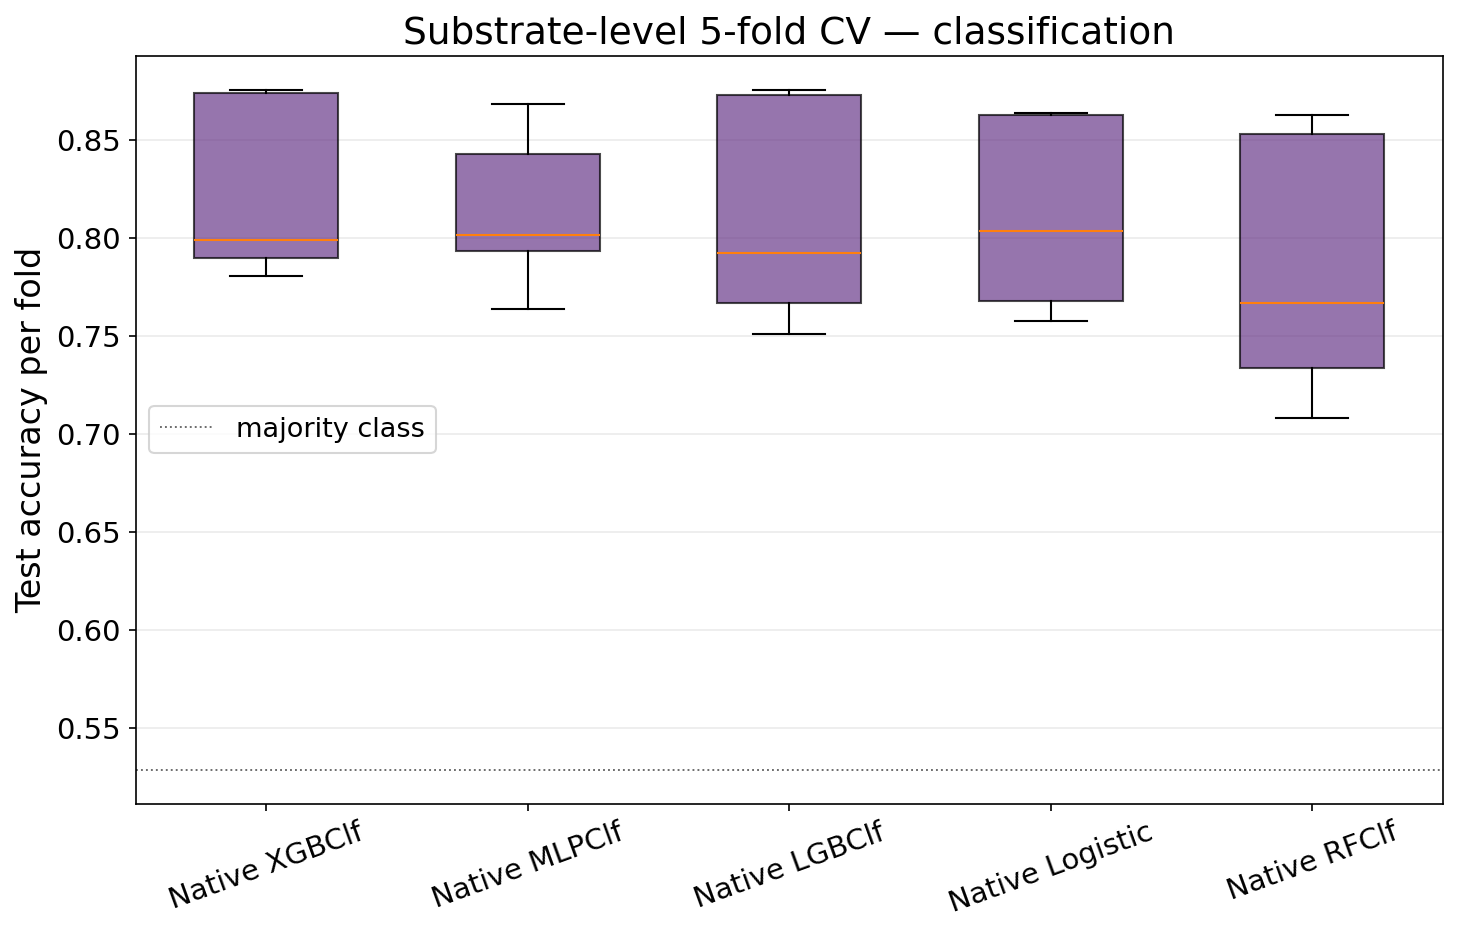
\includegraphics[width=\linewidth,height=0.62\textheight,keepaspectratio]
{kfold_classification.png}
\column{0.43\textwidth}
\textbf{Top results}:
\begin{itemize}
\item Native\_XGBClf: \\ $0.824 \pm 0.047$ acc
\item Native\_LGBClf: \\ $0.812 \pm 0.059$ acc
\item CFA $k$-way: \\ $0.804 \pm 0.038$ acc
\end{itemize}
\textbf{Selection stability}:
\begin{itemize}
\item LGBClf + XGBClf chosen \textbf{5/5 folds}
\end{itemize}
Not a lucky seed.
\end{columns}
\end{frame}

% ── 7. CFA ablation ─────────────────────────────────────────────────────────
\begin{frame}{Does CFA earn its complexity?}
\textbf{Comparison: CFA vs.\ simpler ensemble strategies on the same pool.}
\begin{columns}[T,onlytextwidth]
\column{0.58\textwidth}
\centering
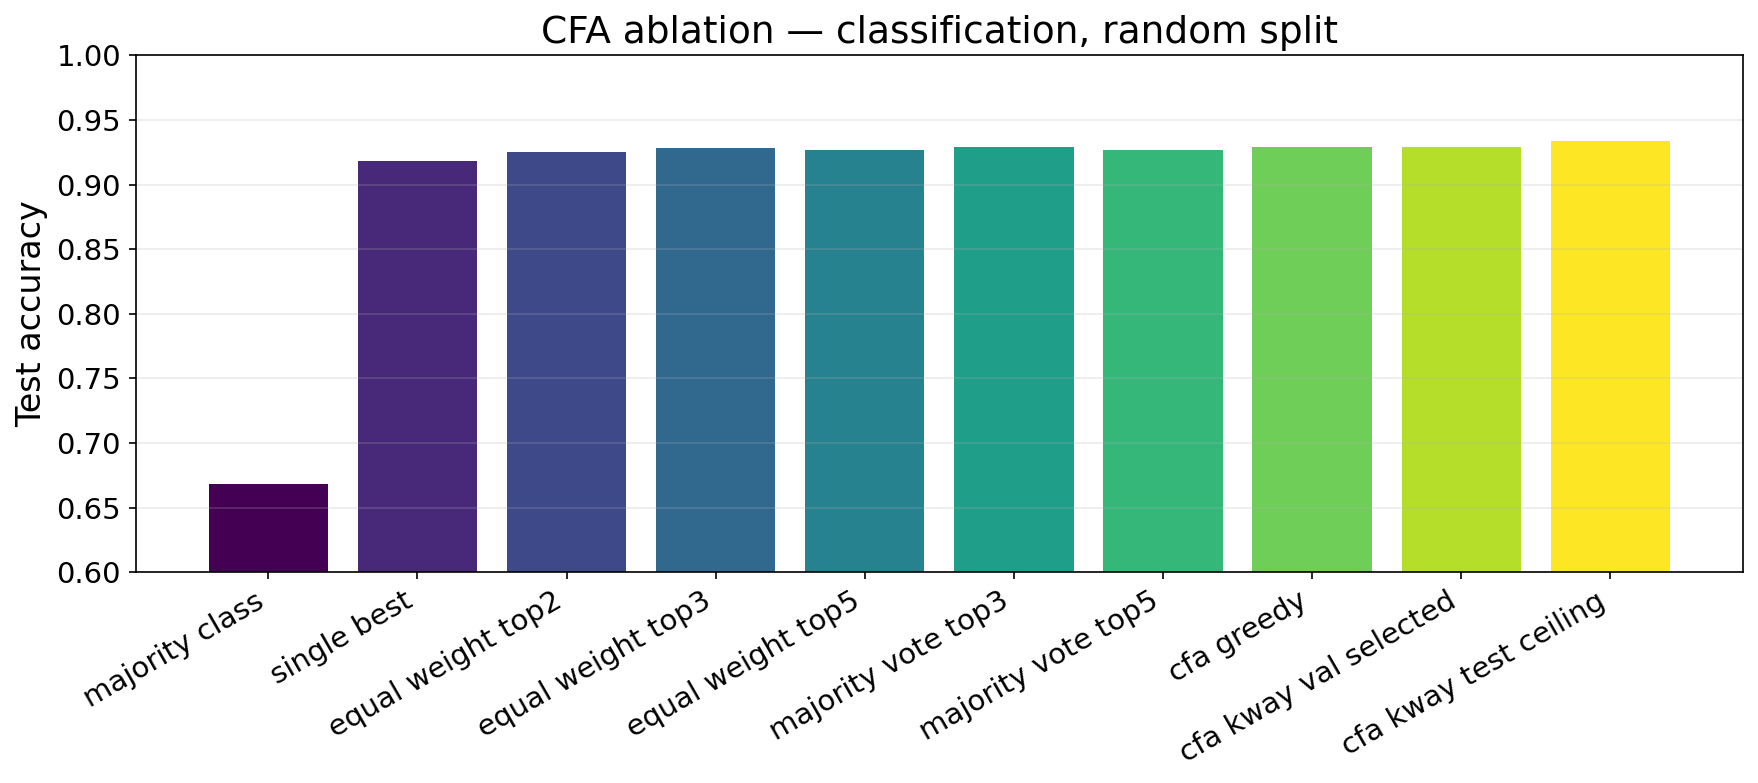
\includegraphics[width=\linewidth,height=0.55\textheight,keepaspectratio]
{ablation_classification_random.png}
\column{0.40\textwidth}
\textbf{Findings:}
\begin{itemize}
\item Random regression: CFA \textbf{+0.012 R$^2$} over equal-weight top-5.
\item Random classification: CFA \textbf{ties} majority-vote-top-3.
\item Scaffold splits: val ($n=10$) too small to rank ensembles.
\end{itemize}
$\implies$ CFA wins on tight regression; ties simple averaging on
large-val classification.
\end{columns}
\end{frame}

% ── 8. Threshold robustness ─────────────────────────────────────────────────
\begin{frame}{Robustness to the success threshold}
The 50\,\% yield threshold is from synthetic-chemistry literature, but
downstream users may care about other cut-offs.
\vspace{0.3cm}
\centering
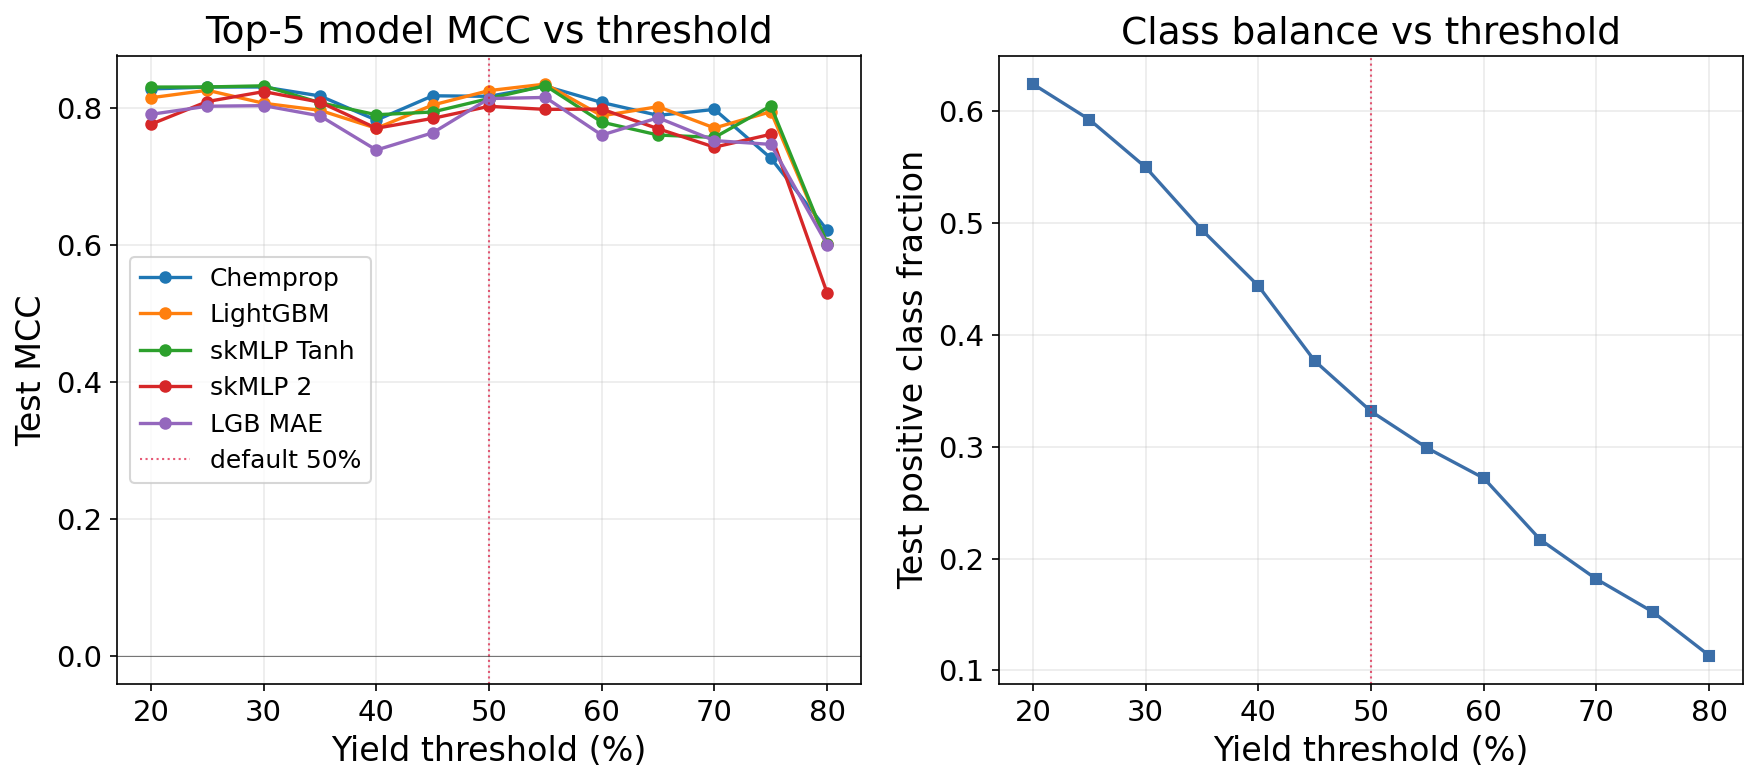
\includegraphics[width=0.95\linewidth,height=0.62\textheight,keepaspectratio]
{threshold_sweep_random.png}
\vspace{0.2cm}
\small Random-split MCC stays $\geq 0.78$ across 50--75\,\% --- the model is
not overfit to the 50\,\% choice.
\end{frame}

% ── 9. Limitations + summary ────────────────────────────────────────────────
\begin{frame}{Summary \& limitations}
\textbf{What we built}
\begin{itemize}
\item 51-model pool $+$ deep chemistry model (Chemprop) $+$ CFA over 6 weighting variants.
\item Two evaluation regimes: random in-distribution; substrate-level 5-fold CV for OOD.
\item Statistical reliability: bootstrap 95\,\% CIs, multi-seed mean$\pm$std,
McNemar tests, CFA ablation, threshold sweep.
\end{itemize}
92\,\% in-dist accuracy, 80\,\% OOD substrate-level accuracy.
\vspace{0.3cm}

\textbf{Honest limitations}
\begin{itemize}
\item Bemis-Murcko scaffold OOD (stricter test, extreme extrapolation):
accuracy drops to 59\,\% with a $n=10$ val that can't rank ensembles.
\item ORD reporter bias: high-yield reactions over-represented; classifier
inherits.
\end{itemize}
\end{frame}

% ── Backup ──────────────────────────────────────────────────────────────────
\appendix

\begin{frame}{Multi-seed reliability}
5 seeds, native classifiers, both splits.
\vspace{0.3cm}
\begin{table}
\small
\begin{tabular}{lrrr}
\toprule
\multicolumn{4}{c}{\textbf{Random split (in-dist)}} \\
Model & Accuracy & MCC & AUC \\
\midrule
Native\_LGBClf & $0.910 \pm 0.010$ & $+0.798 \pm 0.020$ & $0.970 \pm 0.006$ \\
Native\_XGBClf & $0.901 \pm 0.011$ & $+0.776 \pm 0.025$ & $0.966 \pm 0.008$ \\
\midrule
\multicolumn{4}{c}{\textbf{Substrate-level 5-fold CV (OOD)}} \\
Native\_XGBClf & $0.824 \pm 0.047$ & $+0.579 \pm 0.064$ & $0.901 \pm 0.039$ \\
Native\_LGBClf & $0.812 \pm 0.059$ & $+0.551 \pm 0.087$ & $0.897 \pm 0.045$ \\
\bottomrule
\end{tabular}
\end{table}
\end{frame}

\begin{frame}{Native classifier vs thresholded regressor}
\centering
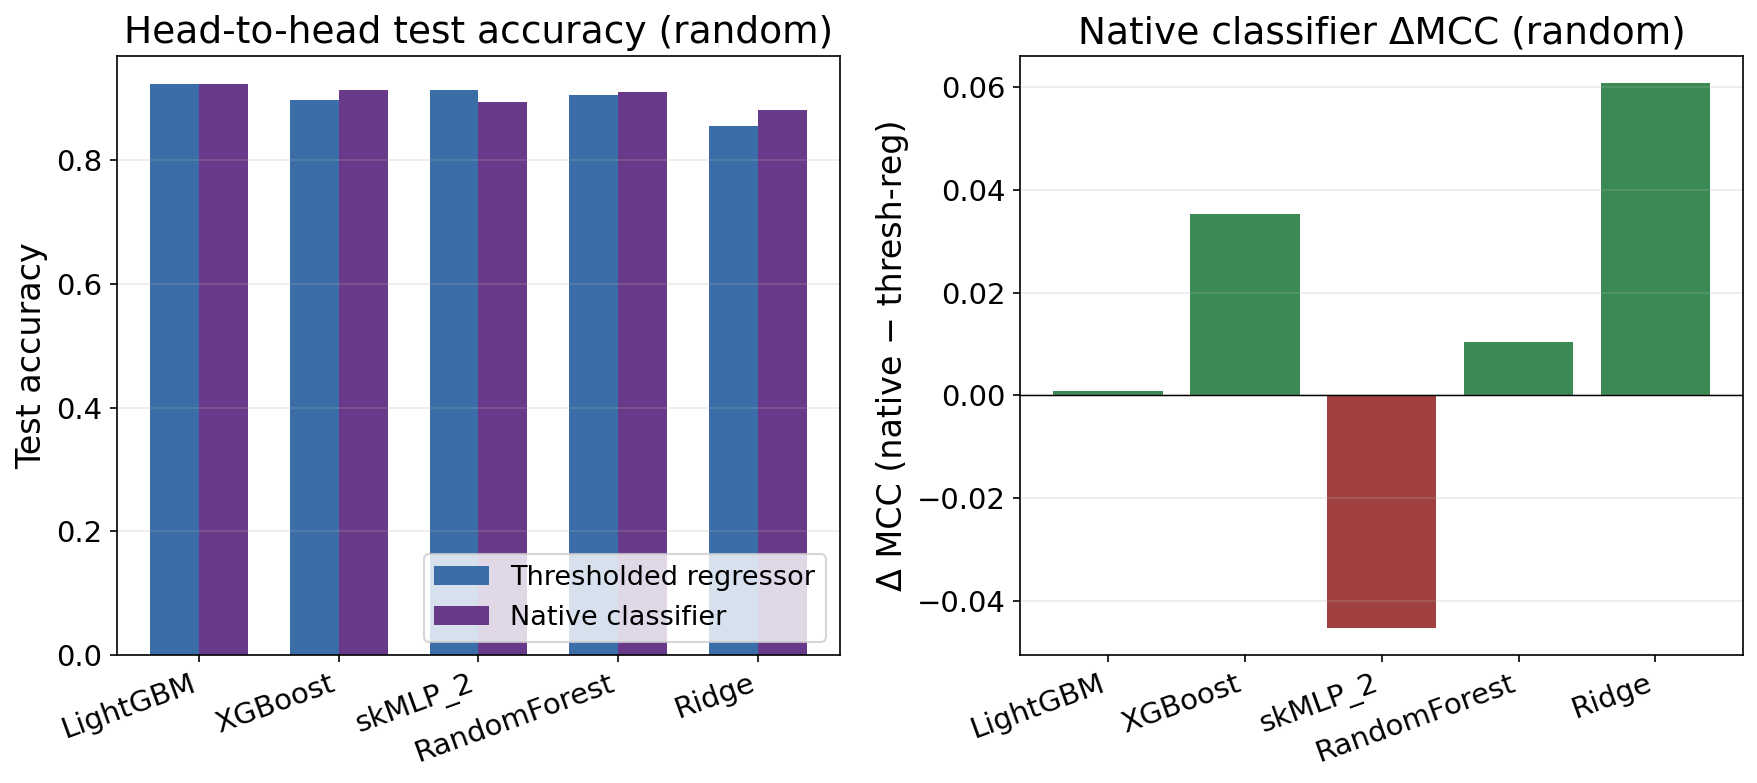
\includegraphics[width=0.9\linewidth,height=0.7\textheight,keepaspectratio]
{native_vs_regressor_random.png}
\end{frame}

\begin{frame}{Rank-score curves}
CFA's signature visualisation: each model's predictions normalised to
$[0,1]$ and sorted descending; oracle = sorted ground truth.
\vspace{0.2cm}
\centering
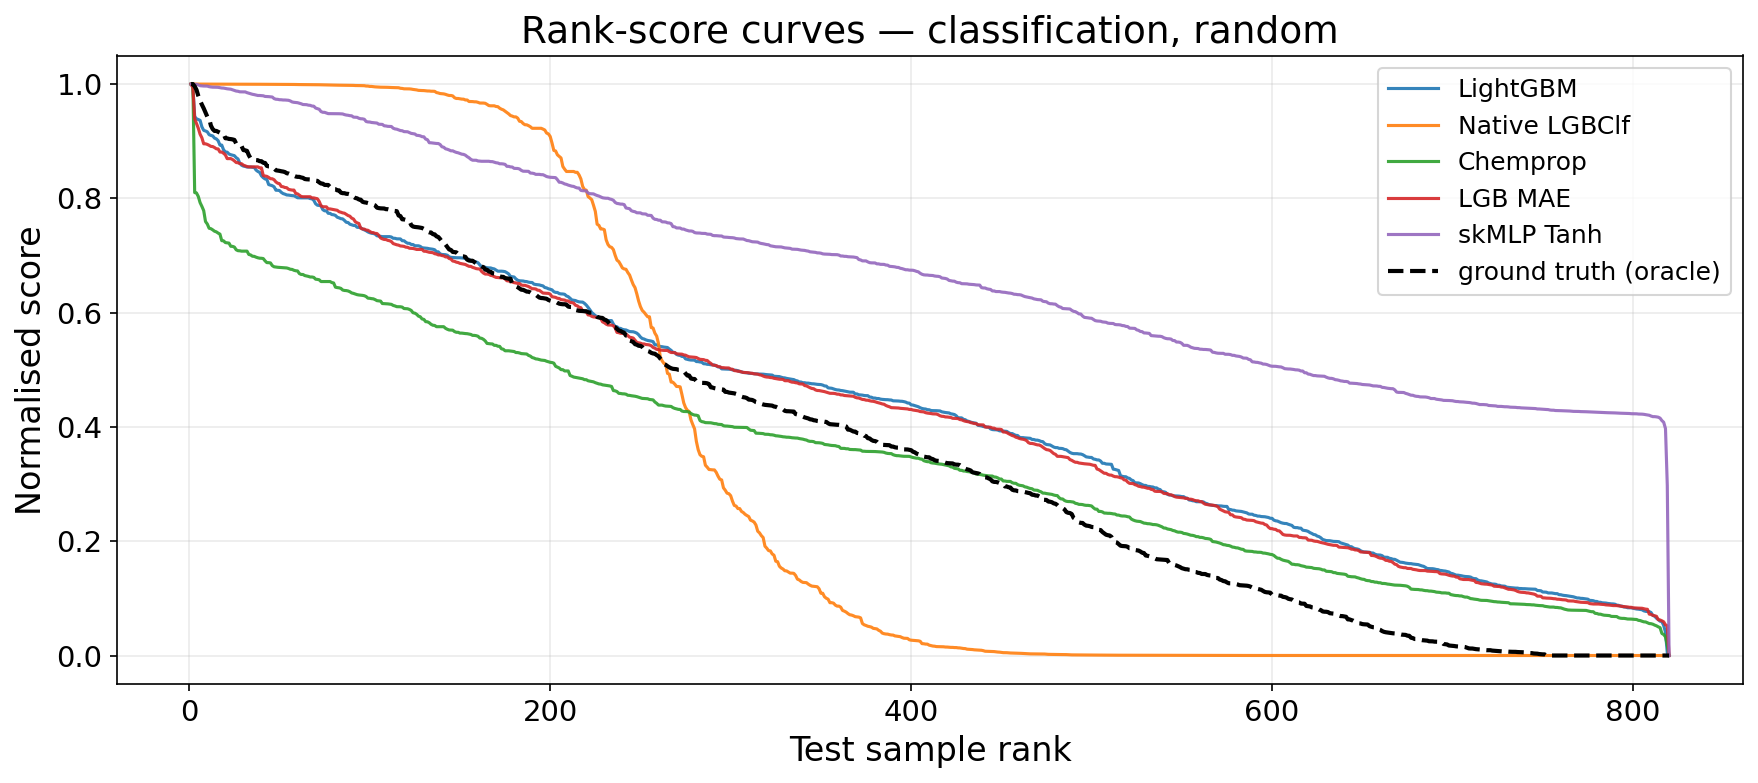
\includegraphics[width=0.85\linewidth,height=0.62\textheight,keepaspectratio]
{rank_score_classification_random.png}
\end{frame}

\begin{frame}{Paired statistical tests}
\textbf{Random classification, McNemar $p$-values:}
\vspace{0.3cm}
\begin{table}
\small
\begin{tabular}{llrrl}
\toprule
A & B & A acc & B acc & McNemar $p$ \\
\midrule
LightGBM       & Native\_LGBClf  & 0.923 & 0.923 & 0.89 (tied) \\
Native\_Logistic & Ridge          & 0.880 & 0.856 & \textbf{0.036} (Native wins) \\
LightGBM       & Chemprop        & 0.923 & 0.918 & 0.67 (tied) \\
Native\_LGBClf & Native\_XGBClf  & 0.923 & 0.913 & 0.29 (tied) \\
\bottomrule
\end{tabular}
\end{table}

\vspace{0.4cm}
\textbf{Scaffold-OOD highlights:} Native classifiers \emph{do} reliably beat
thresholded regressors on the linear family (Logistic > Ridge,
$p = 0.04$); for boosted trees the two are statistically tied.
\end{frame}

\begin{frame}{Confusion matrix}
\centering
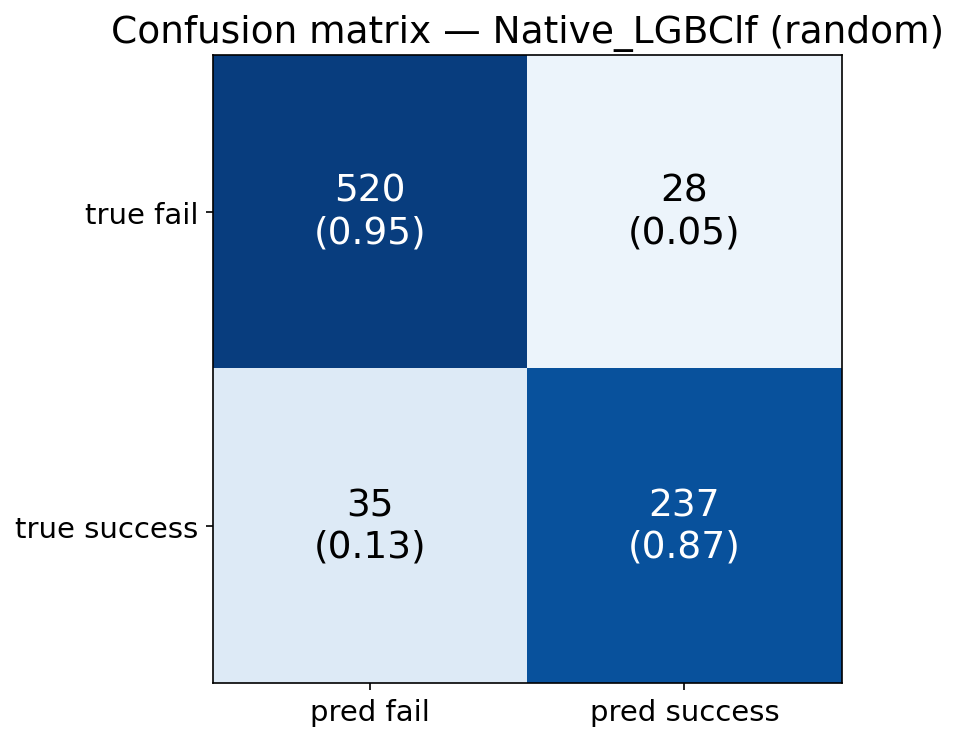
\includegraphics[width=0.5\linewidth,height=0.65\textheight,keepaspectratio]
{confusion_Native_LGBClf_random.png}

\vspace{0.2cm}
\small Native\_LGBClf, random split. Imbalance: 67/33. Errors are roughly
balanced --- not failing on minority class.
\end{frame}

\begin{frame}{Learning curves --- "would more data help?"}
\textbf{Subsample train at 10/30/60/90/100 \%; retrain; evaluate on held-out test.}
\vspace{0.1cm}
\begin{columns}[T,onlytextwidth]
\column{0.5\textwidth}
\centering
\textbf{In-distribution (saturating)}\\[2pt]
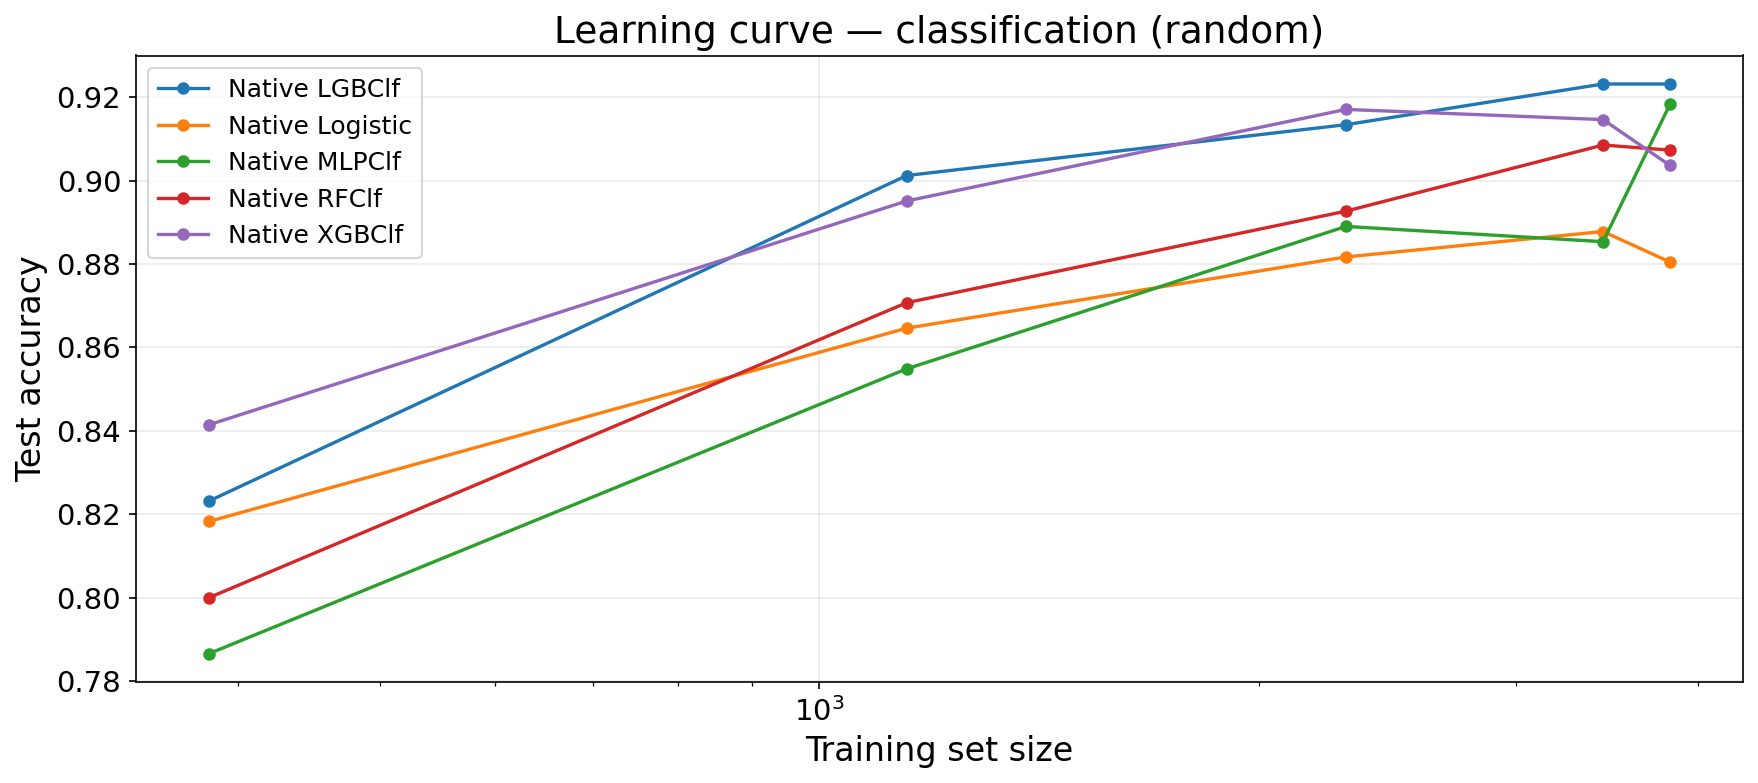
\includegraphics[width=\linewidth,height=0.55\textheight,keepaspectratio]
{learning_curve_classification_random.png}
\column{0.5\textwidth}
\centering
\textbf{Substrate-OOD (still rising)}\\[2pt]
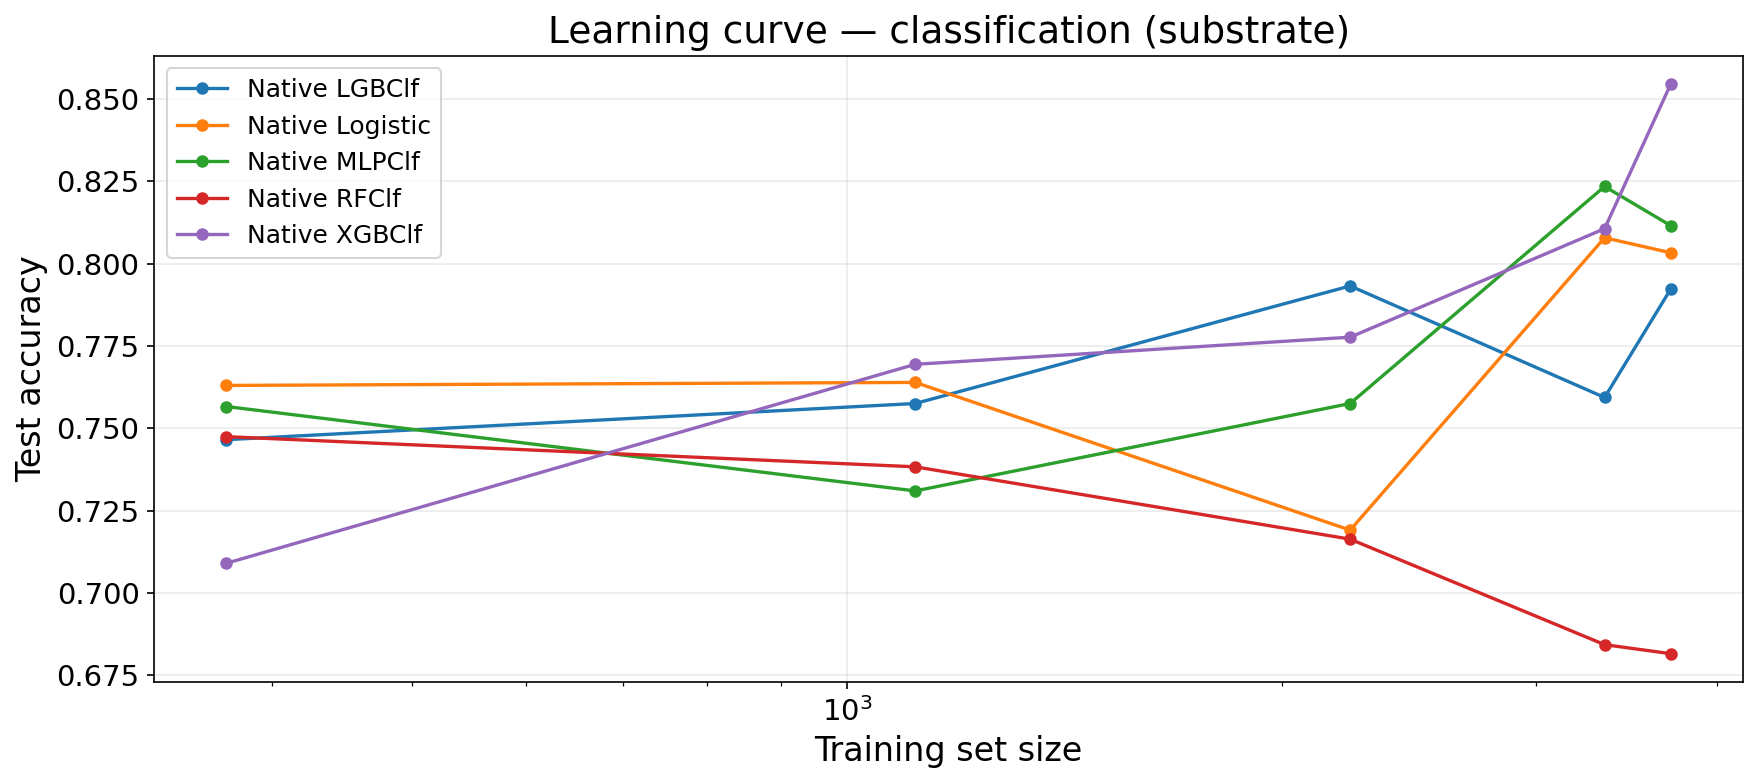
\includegraphics[width=\linewidth,height=0.55\textheight,keepaspectratio]
{learning_curve_classification_substrate.png}
\end{columns}
\vspace{0.1cm}
\small In-distribution curves plateau by 3,800 rows; substrate-level OOD
curves are \emph{still rising} at 100\,\% of available data --- empirical
evidence that more chemistry data would lift OOD accuracy.
\end{frame}

\end{document}
